\documentclass[10pt,a4paper]{article}

% ---------- Page and fonts ----------
\usepackage[a4paper,margin=1.5cm,top=1.3cm,bottom=1.3cm]{geometry}
\usepackage[T1]{fontenc}
\usepackage{mathptmx}                 % Times for text and math
\usepackage[scaled=0.92]{helvet}      % Helvetica for headings
\usepackage{courier}
\usepackage{microtype}
\usepackage{multicol}
\usepackage{enumitem}
\usepackage{booktabs}
\usepackage{tabularx}
\usepackage{titlesec}
\usepackage[dvipsnames]{xcolor}
\usepackage{tikz}
\usetikzlibrary{arrows.meta,positioning,fit}
\usepackage[hidelinks]{hyperref}
\newcommand{\doi}[1]{\href{https://doi.org/#1}{\color{accent}doi:#1}}

\definecolor{accent}{HTML}{1D5C7D}
\definecolor{soft}{HTML}{E4EEF4}
\definecolor{muted}{HTML}{5A6370}

\setlength{\columnsep}{6mm}
\setlength{\parindent}{0pt}
\setlength{\parskip}{3pt}
\pagestyle{empty}

\titleformat{\section}{\sffamily\bfseries\color{accent}\normalsize}{\thesection.}{0.4em}{}
\titlespacing*{\section}{0pt}{5pt}{2pt}
\setlist{nosep,leftmargin=1.3em}

\begin{document}

% ---------- Header ----------
{\sffamily\small\color{accent}\textbf{Term project: Edge AI and IoT Integration}}\\[2pt]
{\large\bfseries SLA-Aware Split Inference with Early Exit for IoT}\\[4pt]
{\sffamily\footnotesize\color{muted}
\textbf{\color{black}Student:} Nguyen Minh Chinh (411221380)\quad
\textbf{\color{black}Course:} CSIE52400 Distributed System, National Dong Hwa University\quad
\textbf{\color{black}Date:} October 1, 2026}\\[-4pt]
{\color{accent}\rule{\textwidth}{1.2pt}}

\vspace{-6pt}
\begin{multicols}{2}

\section{Motivation}
Integrating edge AI with the Internet of Things means bringing deep neural network (DNN) inference to devices such as cameras, drones and wearable sensors, which lack the compute and energy to run DNNs quickly on their own. Offloading raw data to the cloud or an edge server costs bandwidth, adds network latency and fails when connectivity degrades. The best place to run each part of a model therefore changes with network conditions and server load, which makes inference placement a distributed systems problem rather than a purely machine learning one.

\section{Objectives}
\begin{enumerate}
  \item Build a multi-exit DNN that can be split between an IoT device and an edge server.
  \item Design a runtime scheduler that jointly chooses the split point $k$ and the early-exit confidence threshold $\tau$ from measured bandwidth and edge load, to meet a user-defined service-level agreement (SLA), e.g.\ ``p95 latency under 100\,ms, maximise accuracy''.
  \item Support many devices sharing one edge server, and fall back to local inference when the edge fails.
  \item Compare against all-on-device, all-offloaded, split-only and exit-only variants.
\end{enumerate}

\section{Related work}
SPINN~\cite{spinn} co-optimises the DNN split point and the early-exit policy at runtime so that inference adapts to changing network conditions and server load; it is the main basis for this project. Edgent~\cite{edgent} combines device--edge partitioning with model right-sizing to meet a latency deadline. Li et al.~\cite{li2024} study fine-grained partitioning when many IoT devices share edge servers, which motivates the multi-client experiments. CoEdge~\cite{coedge} takes a different approach, splitting a single inference across several cooperating devices; device-to-device cooperation is left as an optional extension. The survey in~\cite{survey} frames split computing and early exiting as a research area.

\section{System design}
\noindent\begin{minipage}{\columnwidth}
\begin{center}
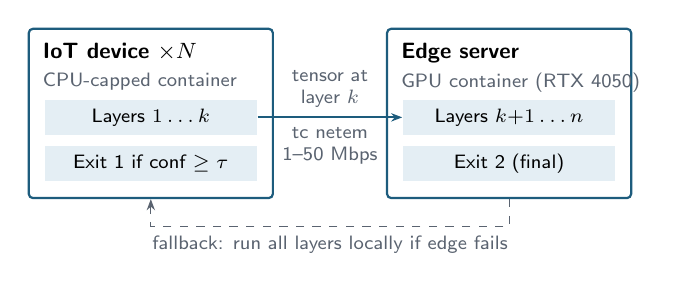
\begin{tikzpicture}[
  font=\sffamily\scriptsize,
  tier/.style={draw=accent,thick,rounded corners=1.5pt,minimum width=3.1cm,minimum height=2.15cm,fill=white},
  blk/.style={fill=soft,minimum width=2.7cm,minimum height=0.45cm,inner sep=1pt},
  arr/.style={-{Stealth[length=4pt]},accent,thick},
  fb/.style={-{Stealth[length=4pt]},muted,dashed}
]
  % device
  \node[tier] (dev) at (0,0) {};
  \node[anchor=north west,font=\sffamily\footnotesize\bfseries] at ([xshift=2pt,yshift=-2pt]dev.north west) {IoT device $\times N$};
  \node[anchor=north west,text=muted] at ([xshift=2pt,yshift=-13pt]dev.north west) {CPU-capped container};
  \node[blk] (d1) at ([yshift=-0.05cm]dev.center) {Layers $1\ldots k$};
  \node[blk,below=0.12cm of d1] (d2) {Exit 1 if conf $\geq \tau$};
  % edge
  \node[tier] (edge) at (4.55,0) {};
  \node[anchor=north west,font=\sffamily\footnotesize\bfseries] at ([xshift=2pt,yshift=-2pt]edge.north west) {Edge server};
  \node[anchor=north west,text=muted] at ([xshift=2pt,yshift=-13pt]edge.north west) {GPU container (RTX 4050)};
  \node[blk] (e1) at ([yshift=-0.05cm]edge.center) {Layers $k{+}1\ldots n$};
  \node[blk,below=0.12cm of e1] (e2) {Exit 2 (final)};
  % link
  \draw[arr] (d1.east) -- node[above,text=muted,align=center]{tensor at\\layer $k$} node[below,text=muted,align=center]{tc netem\\1--50 Mbps} (e1.west);
  % fallback
  \draw[fb] (edge.south) -- ++(0,-0.35) -| node[pos=0.25,below,text=muted]{fallback: run all layers locally if edge fails} (dev.south);
\end{tikzpicture}\\[-2pt]
{\footnotesize\color{muted} Figure 1. Device--edge pipeline; the scheduler sets $k$ and $\tau$ together.}
\end{center}
\end{minipage}\par\vspace{3pt}
Offline, a profiler records per-layer compute time on each tier, per-layer output size, and each exit's accuracy and exit rate at different thresholds. Online, the scheduler reads current bandwidth and edge queue length, predicts latency and accuracy for every $(k,\tau)$ pair, and picks the pair that best meets the SLA. It re-plans when conditions change. Tensors move over gRPC; a heartbeat detects edge failure and triggers local fallback.

\section{Experimental setup}
The testbed is emulated on one laptop (RTX 4050, 6\,GB VRAM) using WSL2 and Docker Compose. Device containers are limited to 0.25 CPU and 512\,MB and pinned to separate cores to approximate a Raspberry Pi; the edge container uses the GPU. \texttt{tc netem} sets bandwidth, delay and loss per link. Workload: MobileNetV2 and ResNet-18 on Imagenette, a 10-class ImageNet subset, at 224$\times$224, with 1--10 concurrent clients and injected edge failures.

\section{Evaluation metrics}
SLA satisfaction rate (share of requests meeting the target), end-to-end latency (mean and p95), throughput, top-1 accuracy, bytes transmitted per inference, device exit rate, time to adapt after a bandwidth change, and recovery time after edge failure.

\section{Timeline}
{\small
\begin{tabularx}{\columnwidth}{@{}l X@{}}
\toprule
\textbf{Weeks} & \textbf{Work} \\
\midrule
4--5   & Literature review, proposal, Docker/GPU testbed \\
6--7   & Baselines, CPU-cap calibration, layer profiling \\
8      & Multi-exit model training, exit accuracy profiling \\
9--11  & Joint $(k,\tau)$ scheduler, SLA modes, runtime re-planning \\
12     & Multi-client scaling and fault tolerance \\
13--14 & Full experiments under varied network and load \\
15     & Buffer: catch-up, re-runs, optional extension \\
16     & Analysis and final report \\
17     & Demo video recording and submission \\
\bottomrule
\end{tabularx}}

\section{Expected outcomes and limitations}
The joint scheduler should meet the SLA for more requests than the split-only and exit-only variants and both static baselines across a range of bandwidths and edge loads, while transmitting less data and staying within a small accuracy margin. Because all nodes share one physical host and the network is emulated, absolute numbers will differ from real deployments; energy is estimated from a model rather than measured. These threats to validity will be discussed in the final report.

\end{multicols}

\vspace{-8pt}
{\color{muted}\rule{\textwidth}{0.4pt}}
\vspace{-14pt}
{\scriptsize
\renewcommand{\refname}{}
\begin{thebibliography}{9}\setlength{\itemsep}{0pt}\setlength{\parskip}{0pt}
\bibitem{spinn} S. Laskaridis, S. I. Venieris, M. Almeida, I. Leontiadis, N. D. Lane, ``SPINN: Synergistic Progressive Inference of Neural Networks over Device and Cloud,'' in \emph{Proc. ACM MobiCom}, 2020. \doi{10.1145/3372224.3419194}
\bibitem{edgent} E. Li, L. Zeng, Z. Zhou, X. Chen, ``Edge AI: On-Demand Accelerating Deep Neural Network Inference via Edge Computing,'' \emph{IEEE Trans. Wireless Communications}, vol.~19, no.~1, 2020. \doi{10.1109/TWC.2019.2946140}
\bibitem{coedge} L. Zeng, X. Chen, Z. Zhou, L. Yang, J. Zhang, ``CoEdge: Cooperative DNN Inference with Adaptive Workload Partitioning over Heterogeneous Edge Devices,'' \emph{IEEE/ACM Trans. Networking}, vol.~29, no.~2, 2021. \doi{10.1109/TNET.2020.3042320}
\bibitem{li2024} H. Li, X. Li, Q. Fan, Q. He, X. Wang, V. C. M. Leung, ``Distributed DNN Inference with Fine-Grained Model Partitioning in Mobile Edge Computing Networks,'' \emph{IEEE Trans. Mobile Computing}, vol.~23, no.~10, 2024. \doi{10.1109/TMC.2024.3357874}
\bibitem{survey} Y. Matsubara, M. Levorato, F. Restuccia, ``Split Computing and Early Exiting for Deep Learning Applications: Survey and Research Challenges,'' \emph{ACM Computing Surveys}, 2022. \doi{10.1145/3527155}
\end{thebibliography}}

\end{document}
